\documentclass[11pt]{report}

\usepackage{fullpage}
\usepackage{graphicx}
\usepackage{hyperref}

\newcommand{\curversion}{1.1.0 Release }



\renewcommand{\familydefault}{\sfdefault}
\title{RMAExpress Users Guide \\ {\small \curversion} \\ {\small \url{http://rmaexpress.bmbolstad.com}}}
\author{B. M. Bolstad \\ bmb@bmbolstad.com}

\begin{document}
\maketitle

\tableofcontents

\chapter{Introduction}

This document is intended as a introductory guide to the RMAExpress \curversion applications. It does not give great details on the underlying algorithms or their implementations. For such materials, the reader is referred to the publications at the conclusion of this document. Although RMAExpress is written to be cross platform, this documentation will concentrate mostly on the Microsoft Windows binaries. Prebuilt binaries of RMAExpress and the associated family of programs are available at the website \url{http://rmaexpress.bmbolstad.com} for both Microsoft Windows and Apple OS X. Additionally source code may be used to build the application on Linux operating systems.  The appearance of windows and menus shown in this document may be different on your operating system.

\section{What is RMAExpress?}

RMAExpress is a cross-platform program which provides methods for producing RMA expression values from Affymetrix CEL files. It has a focus on arrays used for expression analysis. In particular, 3' IVT expression arrays, Exon arrays and the WT Gene arrays can all be processed by RMAExpress.

There are three main applications making up this software package
\begin{itemize}
\item {\bf RMAExpress}: see chapter \ref{chap:RMAExpress}
\item {\bf RMADataConv}: see chapter \ref{chap:RMADataConv}
\item {\bf RMAExpressConsole}: see chapter \ref{chap:RMAExpressConsole}
\end{itemize}

Most users will only need to use the first of these applications, although documentation is provided about all three in this users guide. 

It should be noted that RMAExpress is open source software distributed under the GPL  \url{http://www.gnu.org/copyleft/gpl.html}. Most users will not need to compile their own version of the software and will just use the pre-compiled binaries supplied. However, source code is available at the RMAExpress website and instructions for building it may be found in appendix \ref{chap:building}.

\section{Installing the software}

\subsection{Installing the Software on Microsoft Windows}
To install this software onto a Microsoft Windows operating system first download the installer from the website. Double clicking on the installer binary should open the installer. Installation proceeds as follows:
\begin{enumerate}
\item Depending on your Windows operating system and UAC settings you may get a dialog asking if you wish to allow a program to make changes to your computer.

You should click {\it Yes} on this dialog. Answering {\it No} will close the installer and RMAExpress will not be installed. 

\item If you clicked {\it Yes} then the following dialog is displayed:\\ \\
\begin{center}
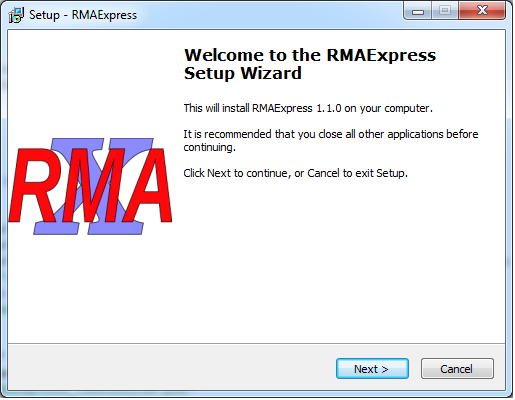
\includegraphics[scale=0.5]{Setup1}
\end{center}
To continue installing click {\it Next}. Choosing {\it Cancel} will quit the installer with no further action taken. 
\item The next stage of the installation is to choose where the application will be installed on your system. This is done using this dialog:
\\
\\
\begin{center}
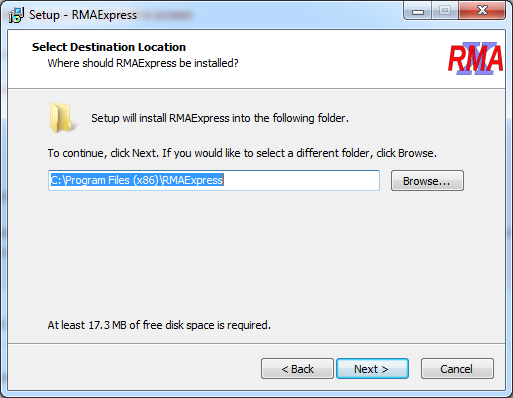
\includegraphics[scale=0.5]{Setup2}
\end{center}
By default it will use {\tt C:/Program Files/RMAExpress} but you may change that to a different location on your system. Click {\it Next} to continue. As before,  {\it Cancel} will quit the installer with no further action taken. \\ \\
\item Now the installer wants to know where you want to put the applications in the Start Menu. By default a new group called {\tt RMAExpress} will be created for the Start menu. It is probably best to just click {\it Next} here: \\ \\ 
\begin{center}
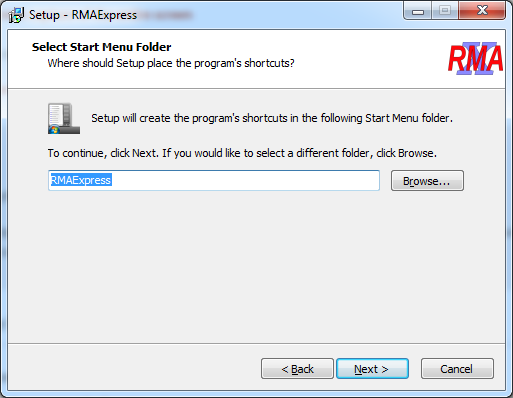
\includegraphics[scale=0.5]{Setup3}
\end{center}

\item The next option you are given is whether or not you want to create desktop icons for RMAExpress and RMADataConv. By default the box is checked. If you do not want these icons to be created unclick the check box. \\ \\
\begin{center}
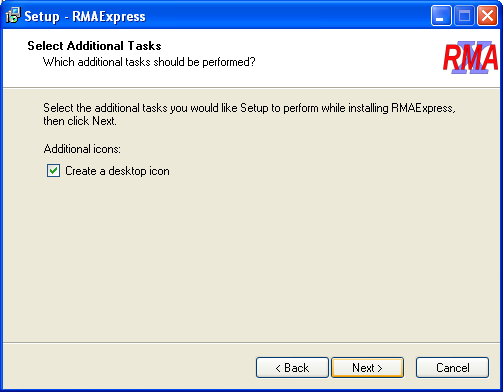
\includegraphics[scale=0.5]{Setup4}\
\end{center}
\item  Finally you are given a brief outline of what the installer will do. Clicking {\it Install} will commence the installation program. Choosing {\it Cancel} will quit the installer with no further action taken.  Note that this is the last possible time to quit the installer without installing the program.
\\ \\ 
\begin{center}
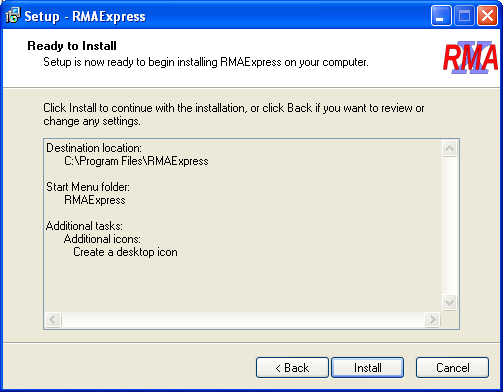
\includegraphics[scale=0.5]{Setup5}
\end{center}

\item A progress bar will show how the installation process is proceeding.\\ \\
\begin{center}
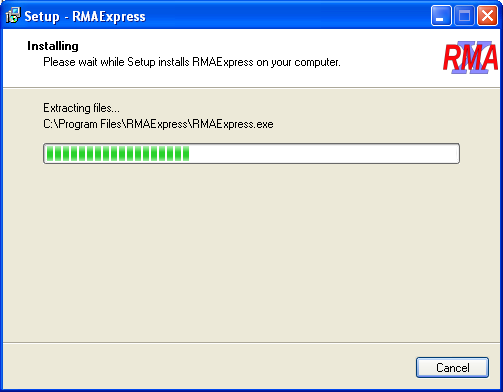
\includegraphics[scale=0.5]{Setup6}
\end{center}
\item After the program is installed a confirmation message is displayed to tell you that the installation completed successfully. If the box is checked then clicking on {\it Finish} will close the installer and launch RMAExpress. If you do not wish to launch RMAExpress immediately then uncheck the box before hitting close. \\ \\
\begin{center}
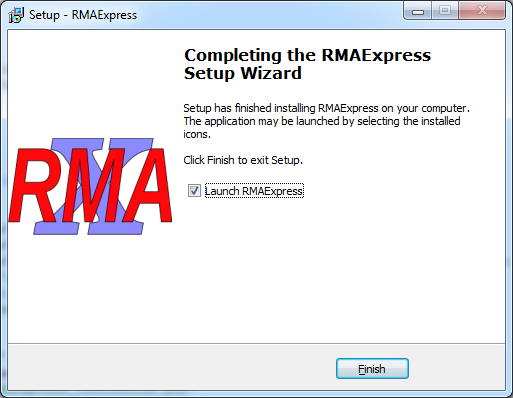
\includegraphics[scale=0.5]{Setup7} 
\end{center}
At this point installation is completed. If you have chosen to install icons they should now be available on your desktop to launch RMAExpress when needed.


\end{enumerate}

\subsection{Installing the Software on Apple OS X}

RMAExpress is provided as a dmg file (Apple Disk Image). Installation of the RMAExpress and RMADataConv applications can be carried out by dragging and dropping the icons onto the Applications alias.

\begin{center}
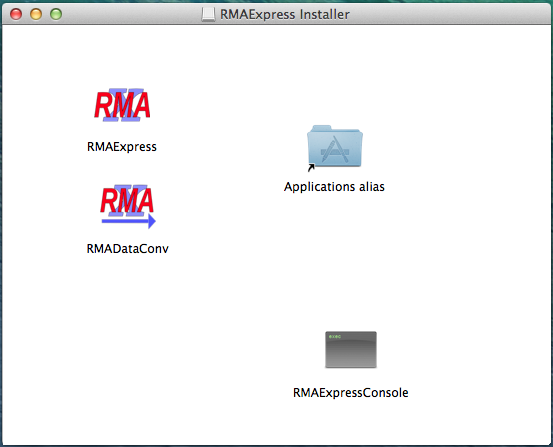
\includegraphics[scale=0.5]{MacOSX_InstallerWindow}
\end{center}

\chapter{RMAExpress: the main application} \label{chap:RMAExpress}

RMAExpress is the main application in the software package. It the primary application in the collection that most users will need to use. The principle functionality is to read raw CEL files, produce RMA expression values and allow a user to conduct some basic QC of their data. 

\section{Exploring RMAExpress}

When you first open RMAExpress you will see a window that looks like the following: \\ \\
\begin{center}
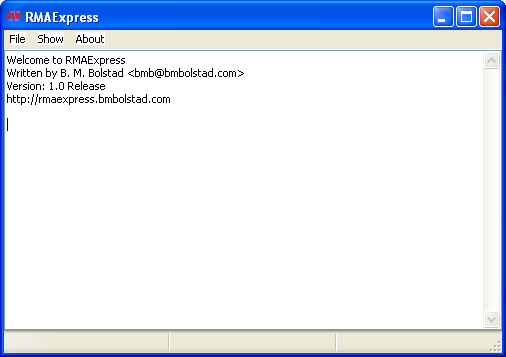
\includegraphics[scale=0.5]{mainwindow}
\end{center}

This application consists of a main window where a log of events is displayed and several menus from which specific commands can be issued. The {\it File} menu is where most commands are issued. It includes commands for: reading in data, computing RMA expression values and writing the results to text files. The {\it Show} menu provides functionality for viewing data, examining residual images and generating quality assessment values. The {\it About} menu gives a dialog box showing the RMAExpress version number.

When the application is initially launched many menu options are not available. In the {\it File} menu the available options are:
\begin{itemize}
\item {\it Read Unprocessed files}: For reading in raw CDF and CEL file data. Note that this will also support reading in CDFRME files generated by RMADataConv 
%\item {\it Read Processed files}: For reading in data which has been processed using the data converter.
\item {\it Output Logfile}: For saving all the messages that appear in the window to a text file.
\item {\it Exit}: For quiting the application.
\end{itemize}
In the {\it Show} menu the available options are\
\begin{itemize}
\item {\it Data}: Which outputs to the main window text messages stating what data is currently loaded into the application. 
\item {\it Preferences}: For setting some preferences. 
\end{itemize}
These two screen-shots show how the menus appear when the program is initially launched:\\ \\
\begin{center}
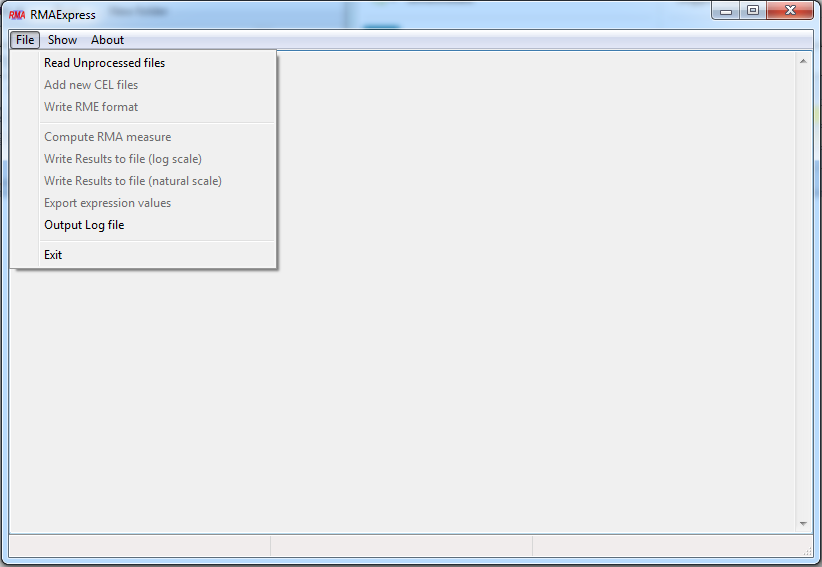
\includegraphics[scale=0.5]{Filemenu1}\\
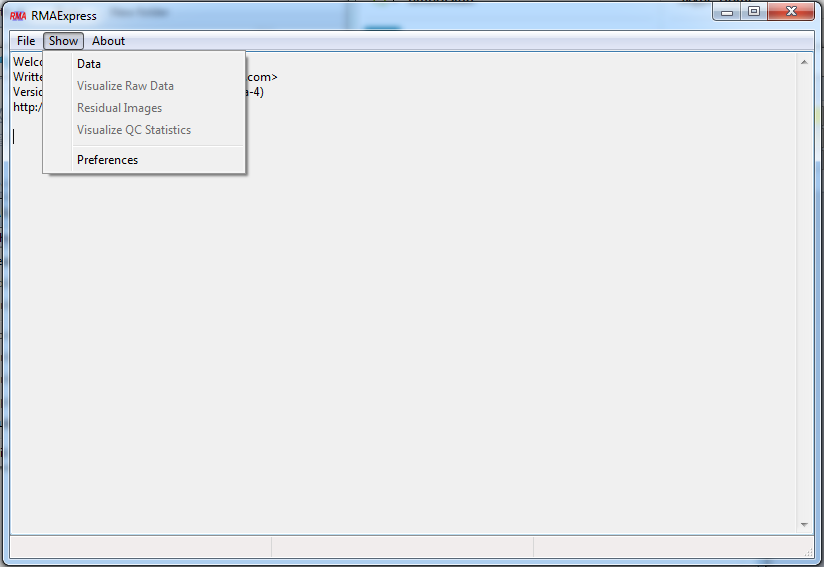
\includegraphics[scale=0.5]{showmenu}
\end{center}

\section{Setting the preferences}

Before you do anything else it is a good idea to set the preferences for the application. To allow the processing of large datasets RMAExpress \curversion buffers data in and out from main memory to disk. The user has some control over this buffering activity, specifically where temporary files are stored and how large the memory buffer is. Choosing {\it Preferences} from the {\it Show} menu will bring up the preferences dialog which will show the current settings: \\ \\
\begin{center}
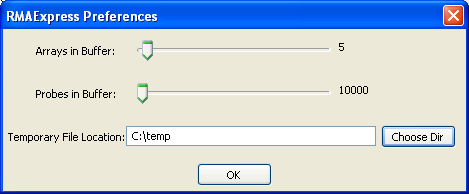
\includegraphics[scale=0.5]{preferenceswindow}
\end{center}
Two sliders control how much data is kept in active memory at any one time. The first slider can be used to control how many arrays will be kept completely in memory. That is every probe intensities for the specified number of arrays will be stored in memory. The second slider controls a slightly different memory buffer. This memory buffer stores a specified number of probes across all chips. For instance if you had this set to 10000 and a dataset with 200 arrays then probe intensities for 10000 probes for all 200 arrays would be kept in memory, irrespective of what arrays were in the first buffer. 

Note that unless you have extremely large amounts of memory you should be conservative in your buffer settings and keep them reasonably sized, since increasing the buffer sizes too much may lead to decreased performance. For users of Windows operating systems best performance is usually achieved by setting the buffer values to their minimums. Increasing these values may actually cause slow downs in performance. Users of Mac OSX and Linux 64 bit operating systems can be more aggressive in their buffer settings.

The final choice the user should make in this dialog box is to specify the location where temporary files should be stored. The user may either type in the full path or click the {\it Choose Dir} button and navigate to the location where temporary files will be written. The chosen location should provide large amounts of disk space. It is very important that the user has read/write permissions to the location chosen. Note that any temporary files created will automatically be deleted when RMAExpress exits.

\section{Loading in data}

The user has two options in the {\it File} menu for loading data. Most users will wish to read data from raw CDF and CEL files. Choosing {\it  Read Unprocessed files} opens this dialog: \\ \\
\begin{center}
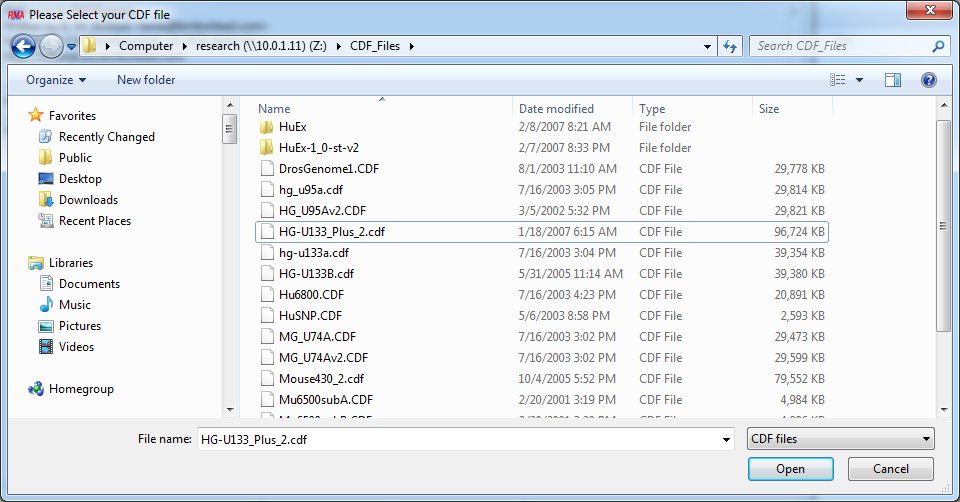
\includegraphics[scale=0.5]{openwindow}
\end{center}
The user should navigate to the location that the appropriate CDF file is stored, select the appropriate CDF file and then click {\it Open}. Clicking {\it Cancel} will stop the process and no data will be loaded. Note that CDFRME (see the RMADataConv documentation) files may also be used.

Next the user should select the CEL files that they wish to load, navigating to and selecting them using this dialog: \\ \\
\begin{center}
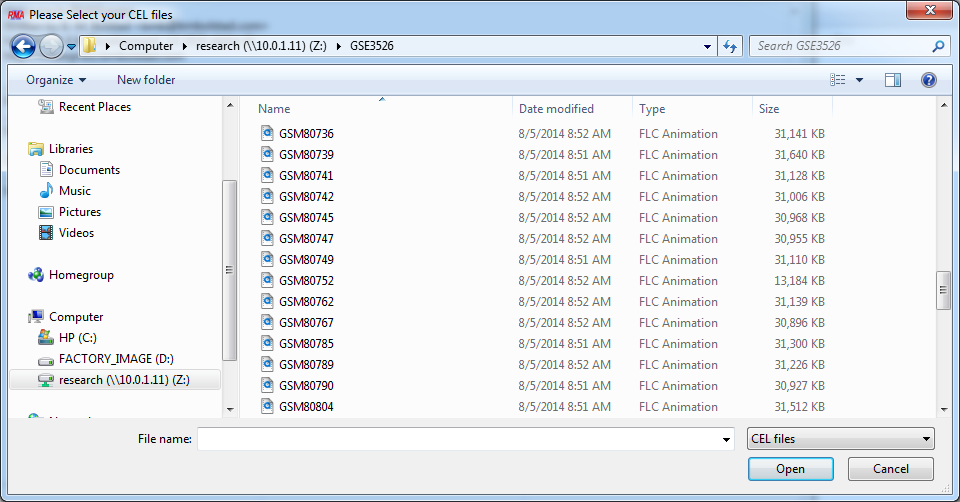
\includegraphics[scale=0.5]{openwindow2}
\end{center}
After the appropriate CEL files have been selected click {\it Open} to begin the process of reading the data into RMAExpress. A series of progress bars will appear on screen letting you know how the process is proceeding.
\begin{center}
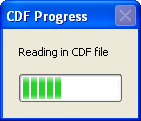
\includegraphics[scale=0.5]{CDFRead}
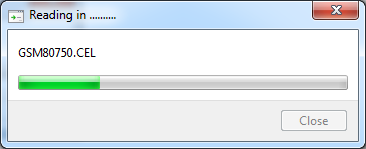
\includegraphics[scale=0.5]{CELRead}

\end{center}



Once the data has been read in several new options are now available for use in the file menu: 
\\ \\ \begin{center}
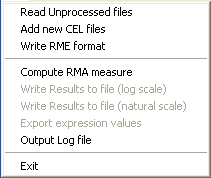
\includegraphics[scale=0.5]{Filemenu2}
\end{center}

Specifically,
\begin{itemize}
\item {\it Add new CEL files}: For reading additional CEL files that were missed in the initial read or stored in another directory.
\item {\it Write RME format}: Output all the currently loaded CEL data in RME files (these are the same format as that produced by RMADataConv).  
\item {\it Compute RMA measure}: This option begins the process of computing RMA expression values from the read in data.
\end{itemize}
 
Also, an additional option may now be chosen from the show menu.
\begin{center}
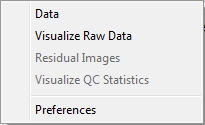
\includegraphics[scale=0.5]{showmenu1}
\end{center}

This item is 
\begin{itemize}
\item {\it Visualize Raw Data}: For looking at boxplots and density plots of the raw unadjusted intensities. 
\end{itemize}
More details about this option can be found in section \ref{sec:visualizerawdata}.

At this point the user should either proceed with their analysis or read additional CEL files using the {\it Add new CEL files} option.


\section{Computing Expression Values}

After data has been read into RMAExpress choosing {\it Compute RMA measure} from the {\it File} menu will the following dialog box to the user: \\ \\
\begin{center}
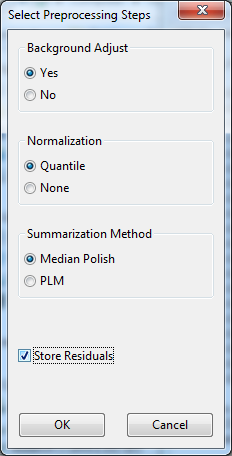
\includegraphics[scale=0.5]{preprocessingstep}
\end{center}
Using this dialog box the user can choose which preprocessing steps to carry out and whether or not to keep the residuals from the modeling procedure. Most users should keep the default background correction ({\it YES}) and normalization ({\it Quantile}) options selected. For the summarization step the user has two choices: {\it Median Polish}, which is the default, and {\it PLM}. These both fit the same summarization model in a robust manner, but do it in different ways. The median polish algorithm is the faster of the two options, and is what gives RMA expression values. Using PLM, which is an abbreviation for {\it probe-level model} will be slower, but it will allow you to examine the QC statistics described in section \ref{sec:PLM QC}. You will not be able to examine these QC quantities if you chose to use the median polish. Checking the {\it Store Residuals} check box will make it possible to visualize chip pseudo-images for quality assessment purposes. These residual images plots can be generated no matter which summarization method was selected. Clicking {\it OK} will start the procedure of computing expression measures. Clicking {\it Cancel} will halt the process.

While RMAExpress is computing expression values a series of dialogs will appear to keep the user updated on progress. It may take some time for this procedure to finish. 

When processing is finished, additional options are now available in the menus. All options should now be available in the file menu and additional options may have become available in the show menu.
\begin{center}
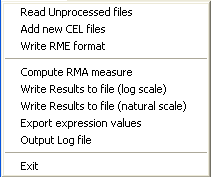
\includegraphics[scale=0.5]{Filemenu3}
\end{center}
In the {\it File} menu new options are:
\begin{itemize}
\item {\it Write Results to file (log scale)}: Output the computed RMA expression values to a text file.
\item {\it Write Results to file (natural scale)}: Output natural scale RMA expression values to a text file.
\item {\it Export expression values}: Export the computed RMA expression values to a binary format file.
\end{itemize}
Note that traditionally RMA expression values are used and expressed in the $\log_2$ scale. However, some external analysis programs may only accept natural scale values. It is for this reason that two different methods which output to text files have been provided. Details about the binary file format can be found in the appendix. The function {\tt ReadRMAExpress} in the BioConductor {\it affyPLM} package will read this output file into R.

In the show menu \\ \\
\begin{center}
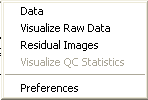
\includegraphics[scale=0.5]{showmenu2}
\end{center}
one new option may be available, provided the user chose to store the residuals when computing RMA expression values by clicking the check box in the pre-processing options dialog. Specifically,
\begin{itemize}
\item {\it Residual Images}: View chip pseudo-images of the residuals
\end{itemize}
The Residual Images option is explained in greater detail in section \ref{sec:resids} of this users guide.

If the user chose the {\it PLM} summarization option then another option will become user selectable from the {\it Show} menu
\begin{center}
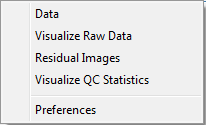
\includegraphics[scale=0.5]{showmenu3}
\end{center}
\begin{itemize}
\item {\it Visualize QC Statistics}: Allows you access to the PLM based NUSE and RLE statistics. 
\end{itemize}
More details about this option can be found in section \ref{sec:PLM QC}.


\section{Visualizing the Raw Data} \label{sec:visualizerawdata}

Choosing {\it  Visualize Raw Data} from the show menu opens the RMAExpress Raw Data Visualizer window. This window looks like this: 
\begin{center}
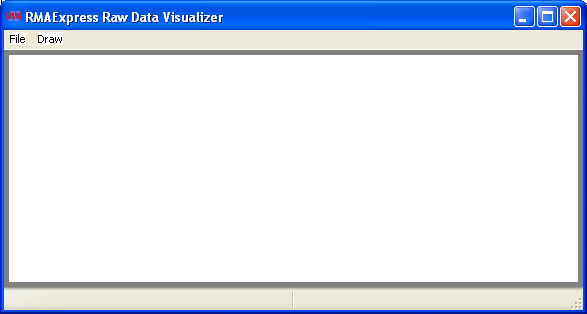
\includegraphics[scale=0.5]{rawdatavisualize1.png}
\end{center}

It has two menus. A {\it File} menu and a {\it Draw} menu:
\begin{center}
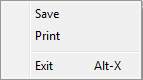
\includegraphics[scale=0.5]{rawdatavisualize2.png}\hspace{0.5in}
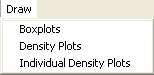
\includegraphics[scale=0.5]{rawdatavisualize3.png}
\end{center}
The {\it File} menu options are:
\begin{itemize}
\item{Save}: Save the current image to a file
\item{Print}: Print the current image
\item{Exit}: Close the Raw Data Visualizer and return to the main RMAExpress window
\end{itemize}



The first option in the {\it Draw} menu is {\it Boxplots}. Selecting this option will draw boxplots of the unadjusted PM intensities, one for each array. For better visualization the PM intensities are $\log_2$ transformed. The following screenshot shows a typical set of boxplots produced : 
\begin{center}
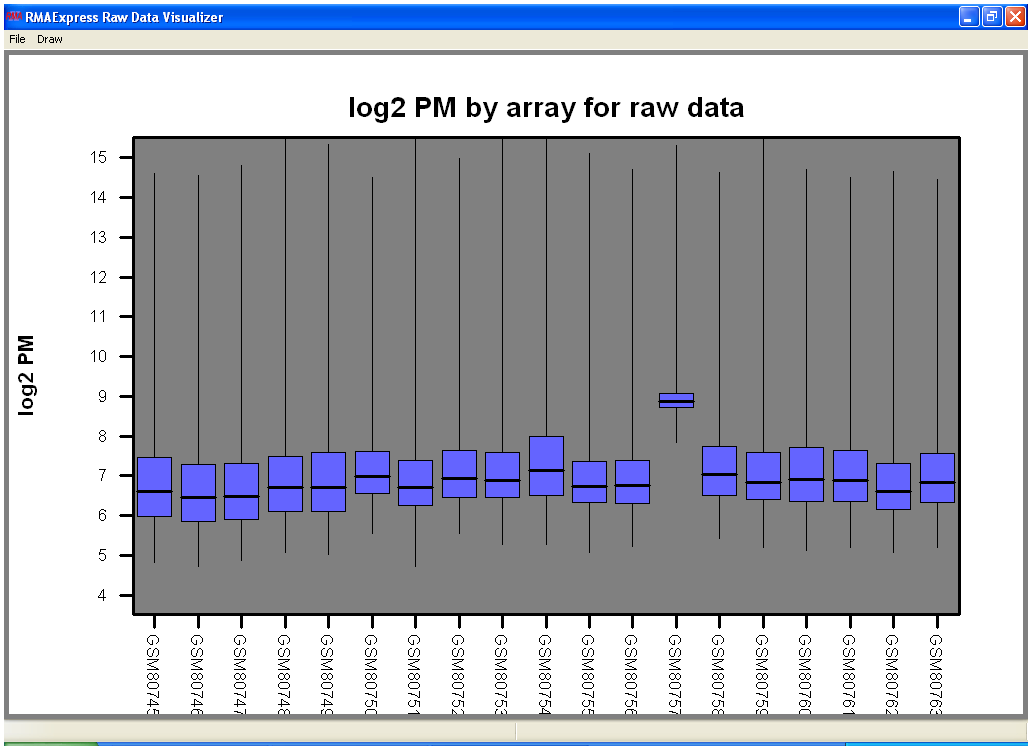
\includegraphics[scale=0.4]{rawdatavisualizeboxplot.png}
\end{center}
Notice that one array was significantly brighter than the other arrays in this dataset.

\clearpage
The second option in the {\it Draw} menu is {\it Density Plots}. Choosing this option produces smoothed density curves of the $\log_2$ PM intensities,  with one curve drawn for each array. A typical set of density plots looks like this:
\begin{center}
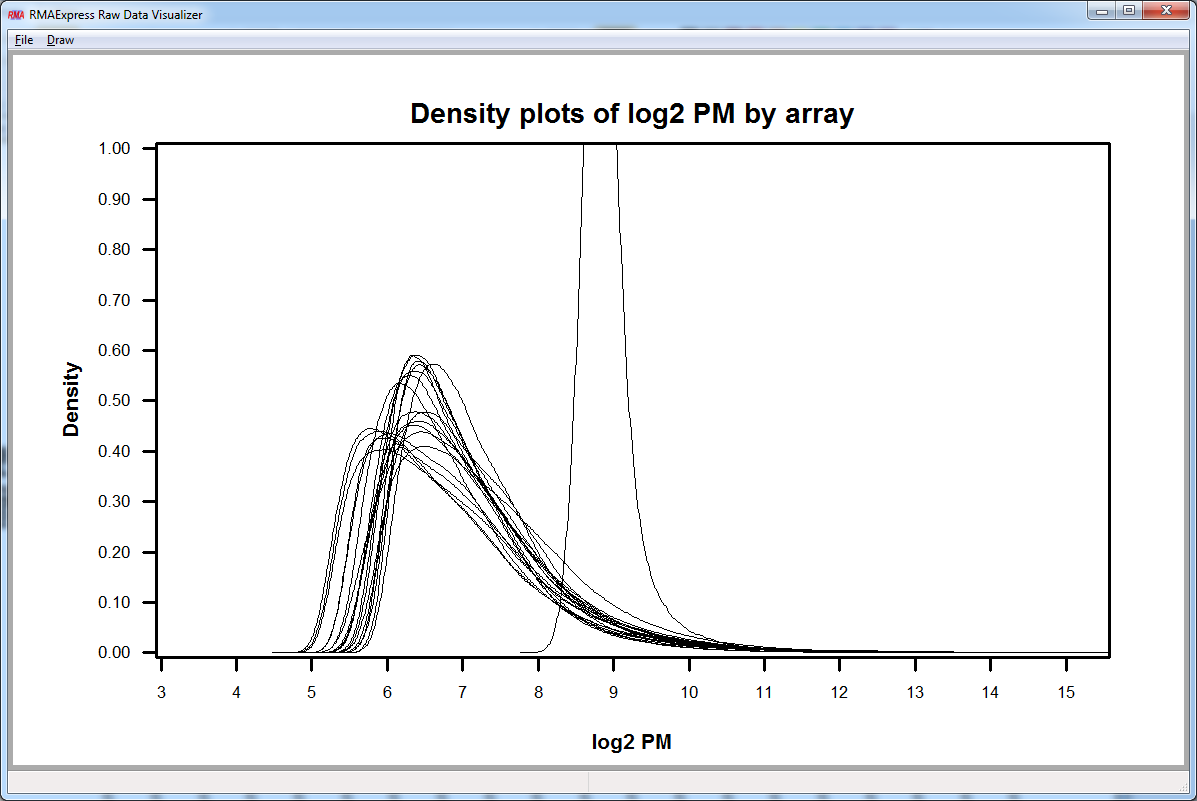
\includegraphics[scale=0.4]{rawdatavisualizedensity.png}
\end{center}
Notice that one array clearly stands out as being different. This may indicate that the data from this array is of poor quality, or it may be that normalization can correct this effect. When using density plots, potential low quality data is often indicated by density curves that are shifted away from the main set of curves or differently shaped.

\clearpage
Because it is difficult to discern which curve belongs to which array the {\it Draw} menu provides a third option {\it Individual Density Plots}. This option produces a density plot for a single array. The user may cycle through the arrays by using the up or down arrow keys. On some platforms the page up and page down buttons may also be used for this purpose.
\begin{center}
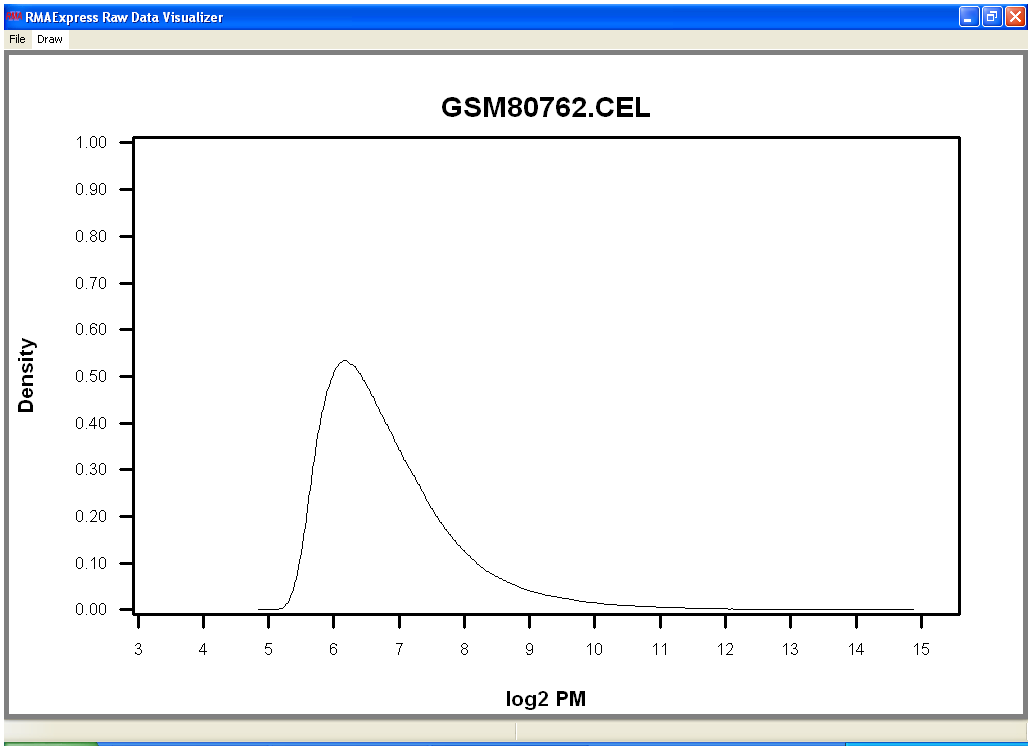
\includegraphics[scale=0.4]{rawdatavisualizedensityindividual.png}
\end{center}

If the {\it Save} option is selected from the {\it File} menu the user will be asked to choose the dimensions and file format of the output file. This is achieved using the following dialog box:
\begin{center}
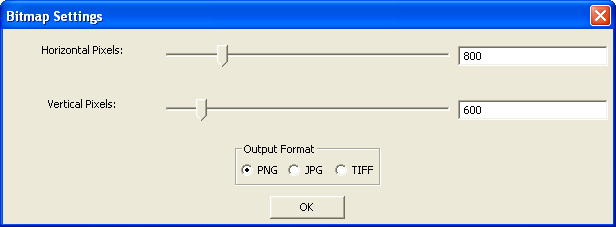
\includegraphics[scale=0.5]{bitmapsettings.png}
\end{center} 

\section{Quality Assessment}


\subsection{Residuals Image} \label{sec:resids}
If the user chose to store residuals when computing expression values then it is possible to visualize the residuals from the RMA procedure on a chip by chip basis. Selecting {\it Residuals Images} from the {\it Show} menu opens the following dialog box: 
\\ \\
\begin{center}
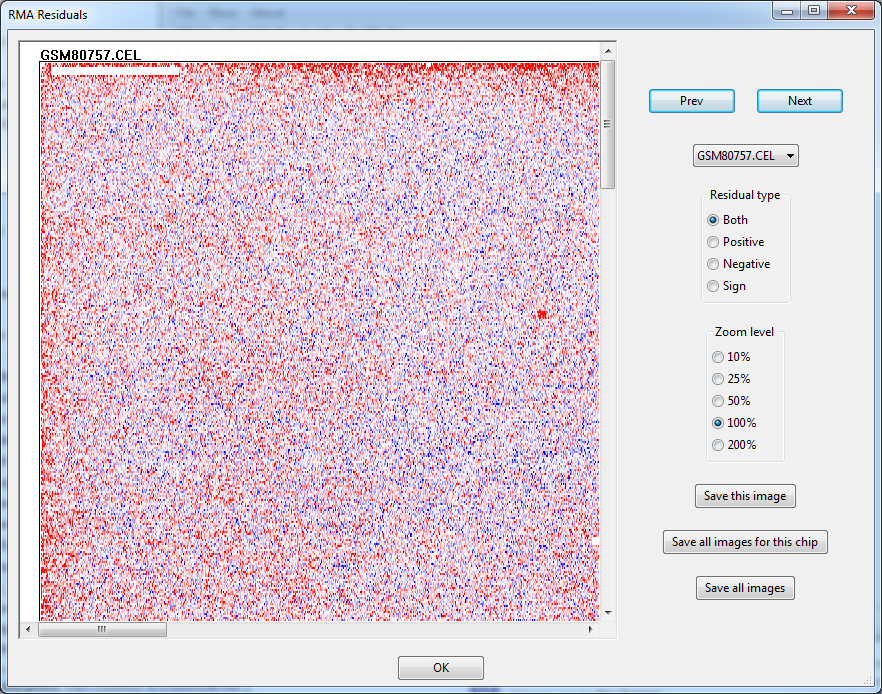
\includegraphics[scale=0.40]{residualsimages}
\end{center}
Chip pseudo-images are displayed in the main pane of this dialog box. Red is used to denote highly positive residuals and blue to denote low negative residuals. White is used for residuals near 0. The intensity of the red or blue designates how far from 0 the residual is.  Poor quality data typically has large intense patches of a single color in distinct regions. In the image shown in this user guide doesn't have any specific artifacts, but because has such intense reds and blues, with little white, it is clear that it is of lesser quality. This user guide is insufficient in length to fully explain how to interpret these images. To get a better feel for typical images, both of good and poor quality, the user is referred to \url{http://PLMImageGallery.bmbolstad.com}.

The user can select which array to visualize by using the {\it Prev} and {\it Next} buttons or by selecting the array by name using the combo box. Radio buttons control which type of image the user is shown. The default setting is {\it Both} which means that both positive and negative residuals are shown. Selecting {\it Positive} or {\it Negative} will show only the red or blue parts of the image respectively. Choosing {\it Sign} means ignore the magnitude of the residual and just color by the sign.  A zoom control allows the size of the residual image to be changed.  Three buttons can be used to save residuals images. The first {\it Save this image} saves the image that is currently drawn. Pushing {\it Save all images for this chip} saves the residuals, positive residuals, negative residuals and sign of residuals images for the current array. Finally using {\it Save all images} produces all of the images for all of the arrays.
\begin{center}
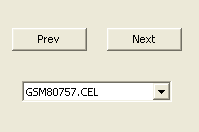
\includegraphics[scale=0.5]{residualsimagescontrol1.png}\hspace{0.5in}
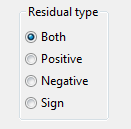
\includegraphics[scale=0.5]{residualsimagescontrol2.png}\\ \vspace{0.2in}
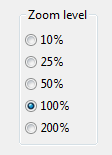
\includegraphics[scale=0.5]{residualsimagescontrol3.png}\hspace{0.5in}
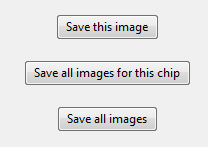
\includegraphics[scale=0.5]{residualsimagescontrol4.png}
\end{center}

Clicking the {\it OK} button will close the Residual images window.

\subsection{PLM based quality assessment} \label{sec:PLM QC}

Choosing {\it  Visualize QC Statistics} from the show menu opens the RMAExpress QC Statistics Visualizer window. This window looks like this: 
\begin{center}
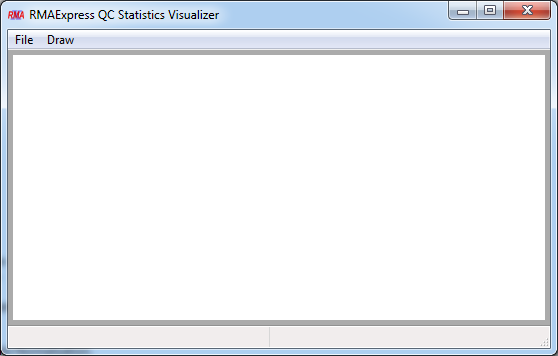
\includegraphics[scale=0.5]{QCVisualize1.png}
\end{center}

It has two menus. The {\it File} menu is for saving output to files and {\it Draw} menu for selecting possible plots. Both revolve around the two main PLM based quality statistics: Normalized Unscaled Standard Error (NUSE) and Relative Log Expression (RLE). These are the current options in the menus:
\begin{center}
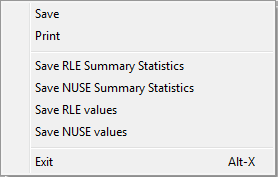
\includegraphics[scale=0.5]{QCVisualize2.png}\hspace{0.5in}
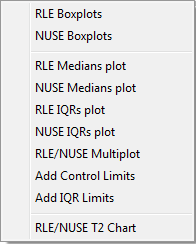
\includegraphics[scale=0.5]{QCVisualize3.png} \\
\end{center}

The {\it File} menu options are:
\begin{itemize}
\item{Save}: Save the current image to a file
\item{Print}: Print the current image
\item{Save RLE Summary Statistics}: Save a summary table to tab delimited text file of the RLE values
\item{Save NUSE Summary Statistics}: Save a summary table to tab delimited text file of the NUSE values
\item{Save RLE Values}: Save RLE values to a tab delimited text file
\item{Save NUSE Values}: Save NUSE values to a tab delimited text file
\item{Exit}: Close the QC Statistics Visualizer and return to the main RMAExpress window
\end{itemize}

There are three different options in the {\it Draw} menu for visualizing the RLE statistic. The first {\it RLE Boxplots} draws boxplots of RLE values, one for each array. Low quality arrays will have greater spreads, or will not be centered near 0. A closer look at the medians can be found by looking at {\it RLE Medians plot}. A third plot shows the RLE IQRs. The following three screenshots show these plots.
\begin{center}
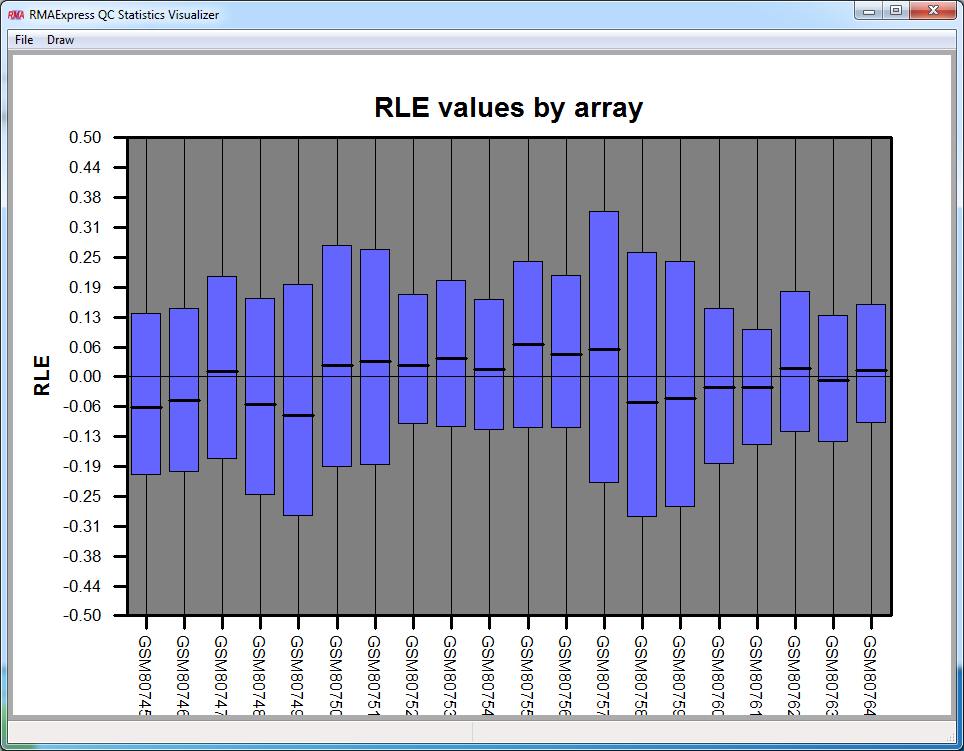
\includegraphics[scale=0.4]{RLEBoxplot.png}\\
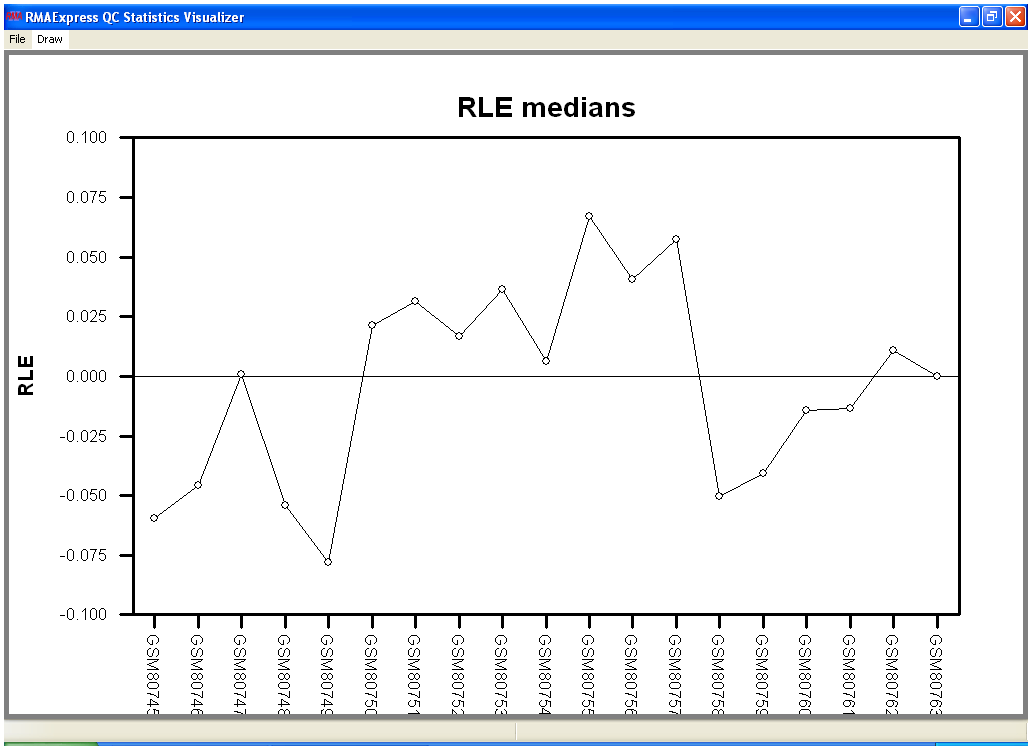
\includegraphics[scale=0.4]{RLEMedians.png}\\
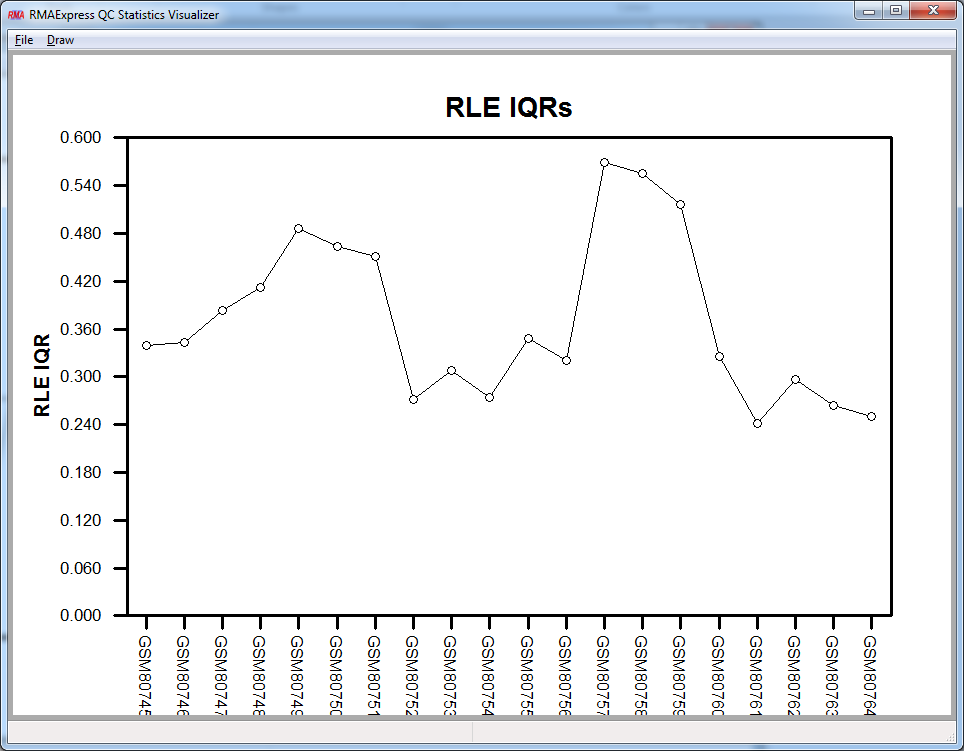
\includegraphics[scale=0.4]{RLEIQRs.png}\\
\end{center}


The {\it Draw} menu also provides three similar options for the NUSE statistic. The first {\it NUSE Boxplots} draws boxplots of the NUSE values. Low quality data will have greater spread or be not centered around 1. The following three screenshots show these plots.
\begin{center}
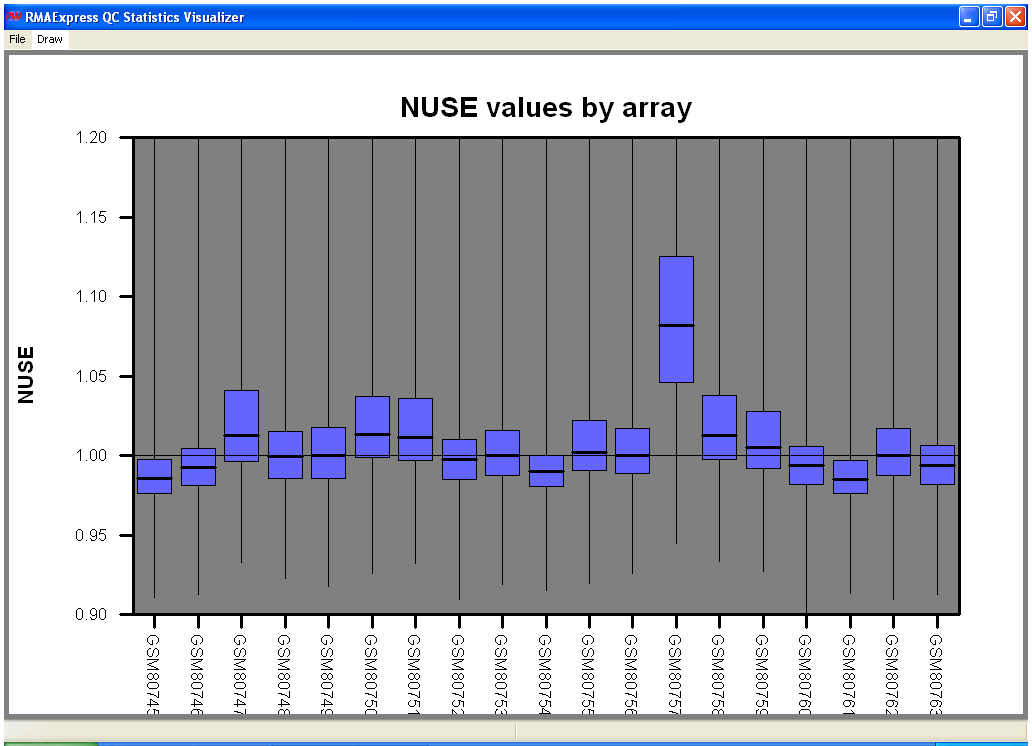
\includegraphics[scale=0.4]{NUSEBoxplot.png}\\
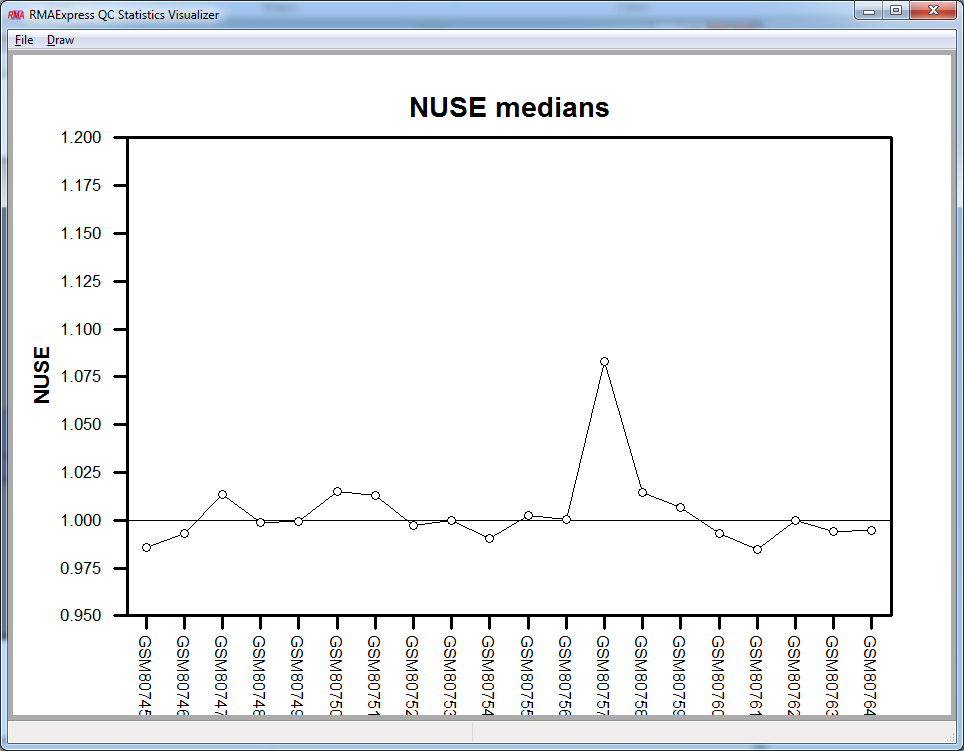
\includegraphics[scale=0.4]{NUSEMedians.png}\\
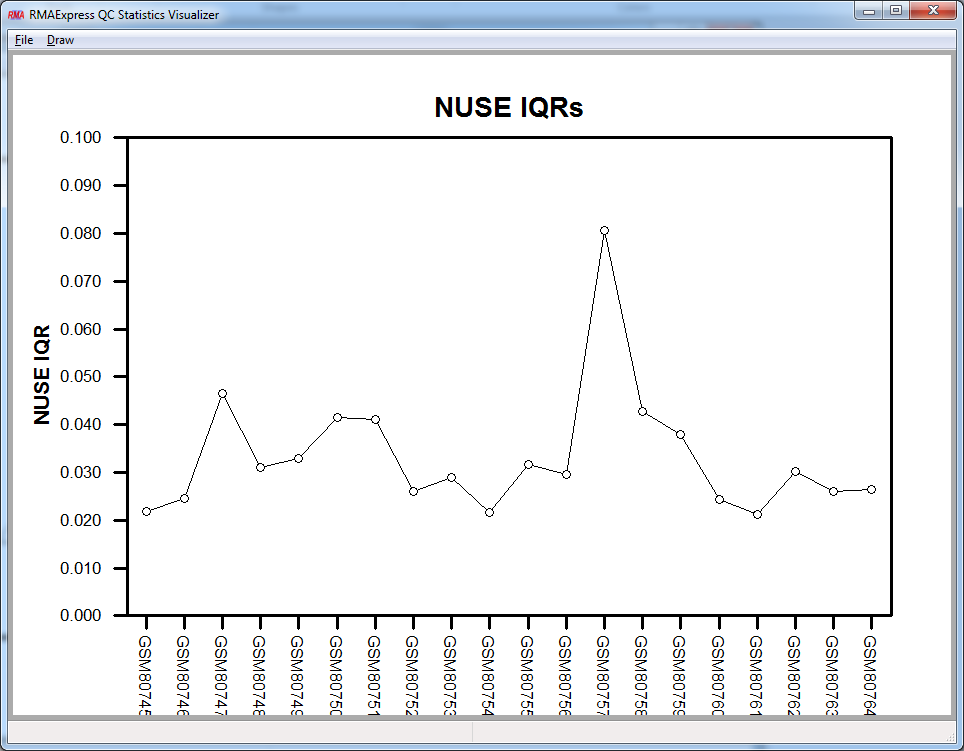
\includegraphics[scale=0.4]{NUSEIQRs.png}\\
\end{center}

One array is clearly of lower quality based on the NUSE plots. This corresponds to the same array discussed in the residuals images section, and also shown in the visualizing raw data section of this user guide.

RMAExpress also provides QC cutoffs that may be applied to the RLE and NUSE single summary plots. These may be triggered by selecting the {\it Add Control Limits} and {\it Add IQR Limits} options.in the {\it Draw} menu. The {\it Add Control Limits} option produces upper and lower control limits that are derived using the methodology for XmR control charts. Blue lines are used to indicate these control limits. he {\it Add IQR Limits} option produces control limits derived based on normal boxplot outlier identification rules. Specifically, the limits are at 1.5*IQR above the upper quartile and 1.5*!QR below the lower quartile. The IQR Limits are drawn using green lines. Note that the user should use the control limits when attempting to identify lower quality arrays, but there are not hard boundaries and should only be considered indicative of arrays for further investigation. Note that the control limit options require the dataset include at least 6 arrays.

In most datasets there is some degree of correlation exists between the RLE and NUSE summary values. The {\it RLE/NUSE Multiplot} option in the {\it Draw} menus combines plots for the four QC summary values together into a single plot. An example plot is shown here (with both types of control limits shown).
\begin{center}
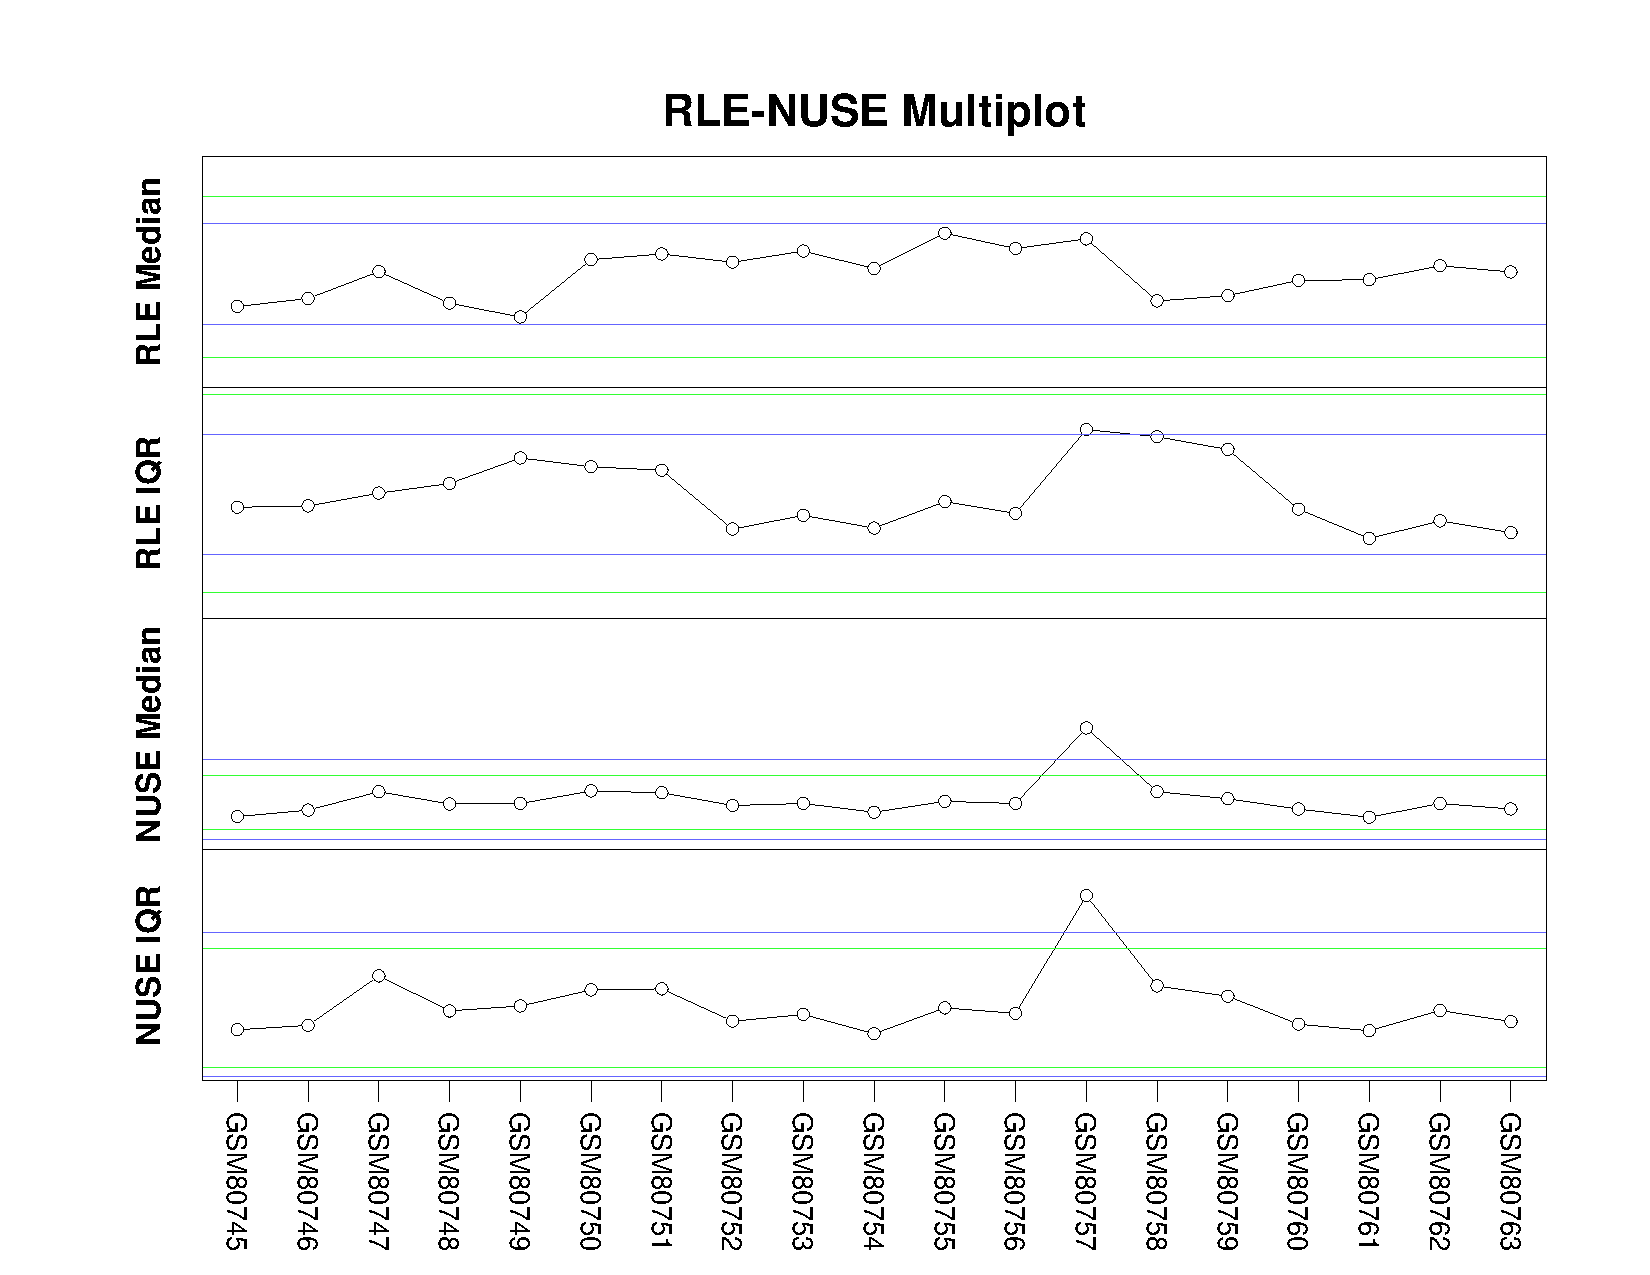
\includegraphics[scale=0.4]{RLENUSEMultiplot_New.pdf}
\end{center}
One array falls well outside the control limits for both NUSE metrics and and is borderline on the RLE IQR plot.

Another QC method is to reduce the multiple RLE and NUSE summaries down to a single number. The {\it RLE-NUSE T2} is one such multivariate statistic. This option is only available when 6 or more arrays are analysed together. The following shows the plot created when the {\it RLE-NUSE T2} option is selected.
\begin{center}
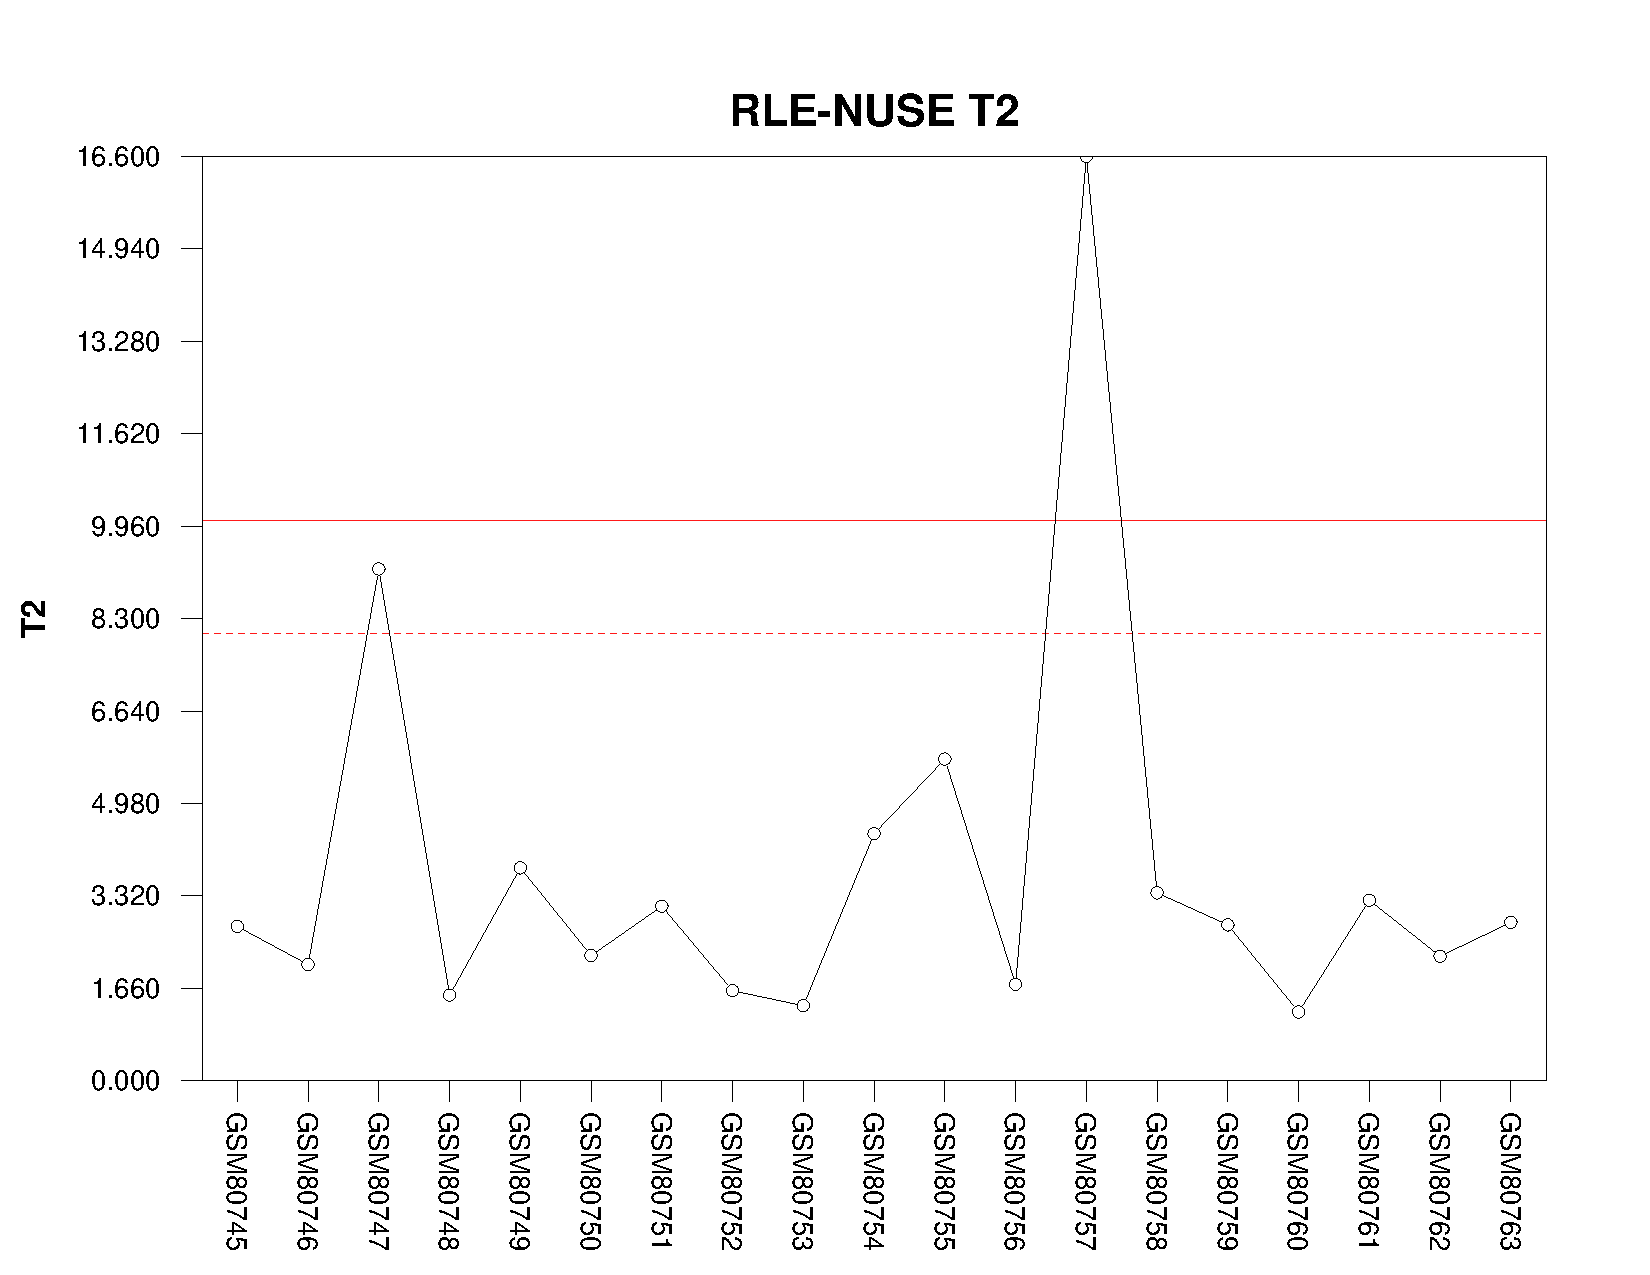
\includegraphics[scale=0.4]{RLE_NUSE_T2.pdf}
\end{center}
Two control limits are shown on this plot. A red dotted line indicates a 95\% cutoff and the solid red line is a 99\% cutoff. Expression values for arrays exceeding the 99\% cutoff should be removed from down stream analysis. Arrays which only exceed the 95\% cutoff warrant further investigation.


Note that the control limits drawn by RMAExpress in the QC statistic visualizer work best when 20 or more arrays are analyzed together.


\chapter{RMADataConv: the data converter} \label{chap:RMADataConv}

RMADataConv is an application for converting CDF and CEL files to an intermediate format that may be read into RMAExpress. Most users will not need to use it since the RMAExpress application supports CDF and CEL files natively. However, the data converter is still useful in some circumstances. This section explains the RMADataConv application and some of its uses. % Note that RME files can be read into RMAExpress using the {\it Read Processed files} option in the {\it File} menu.

\section{The main dialog}

The data converter is a dialog based application. When you launch RMADataConv you are presented with this main dialog box: 
\begin{center}
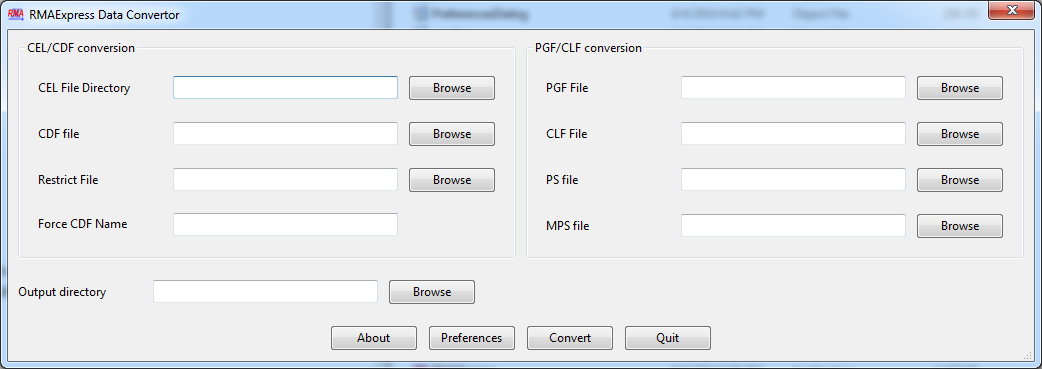
\includegraphics[scale=0.45]{DataConvertor.png}
\end{center}

There are two main groupings of fields, corresponding to the two main file conversion processes. These are for
\begin{itemize}
\item{\it CEL/CDF conversion}: For converting CDF and CEL files into CDFRME and RME format files.
\item{\it PGF/CLF conversion}: Converting PGF/CLF files into CDFRME format files
\end{itemize}

\begin{itemize}
\item {\it Output directory}: The location to store RME files when processed. This field is mandatory for all work flows
\end{itemize}

For CEL/CDF file conversion there are four main fields into which the user can enter text or file paths. These include
\begin{itemize}
\item {\it CEL File Directory}: A directory containing CEL files to be converted into RME format files.
\item {\it CDF File}: A CDF file to be converted into RME format
\item {\it Restrict File}: A file containing probeset names, 1 per line
\item {\it Force CDF Name}: A string specifying how the CDF information should be identified 
\end{itemize}

For PGF/CLF file conversion there are four main fields into which the user can enter text or file paths. Currently two of these are disabled. These include
\begin{itemize}
\item {\it PGF File}: Location of PGF format file
\item {\it CLF File}: Location of CLF format file
\item {\it PS file}: Location of PS file
\item {\it MPS file}: Location of MPS file
\end{itemize}


Note that typically only some of these fields need to be filled for a conversion job. There are also four main buttons
\begin{itemize}
\item {\it About}: Show version number of RMADataConv
\item {\it Preferences}: Set preferences about buffering.
\item {\it Convert}: Start the process of converting to RME format files
\item {\it Quit}: For quiting RMADataConv
\end{itemize}

\section{Turning PGF and CLF files into CDFRME files}

For some array types there are no CDF files supplied by Affymetrix. Primarily these are Exon and WT Gene array (including HTA arrays). For these array types the PGF and CLF files should be used and converted into an appropriate CDFRME file. The RMADataConv application is designed to handle this process. In particular, you should specify the PGF and CLF files in the appropriate fields. The {\it Output directory} field should specify the location to store the output CDFRME file. Clicking {\it Convert} will start the conversion process. When it finishes you should find the CDFRME files in the location specified. A CDFRME file may be used interchangeably with a CDF file in the main RMAExpress application.

The naming convention for the CDFRME file that is produced is as follows: 
\begin{verbatim}
lib_set_name.lib_set_version_pgfclf.CDFRME 
\end{verbatim}
so for example 
\begin{verbatim}
HuEx-1_0-st.r2_pgfclf.CDFRME
\end{verbatim}

Affymetrix provides unsupported CDF files for the Exon arrays (at the time at which this manual was written). While RMAExpress may work with these CDF files, they are also to be considered unsupported (ie use at your own risk).


\subsection{Using PS files}

In some cases rather than summarizing all exons, only RMA values for certain subsets of exons will be desired. Affymetrix classifies Exons into three sets: core, extended and full. Each set encompasses a greater number of exons. PS files may be found on the Affymetrix website. If this is specified in the {\it PS file} field along with appropriate CLF and PGF files, then the conversion process will produce a CDFRME file containing only the specified exons. 

The naming convention for the CDFRME file that is produced is as follows: 
\begin{verbatim}
lib_set_name.lib_set_version_ps_psfilename.CDFRME
\end{verbatim}
so for example 
\begin{verbatim}
HuEx-1_0-st.r2_ps_HuEx-1_0-st-v2.r2.dt1.hg18.full.CDFRME
\end{verbatim}

\subsection{Using MPS files}

It is also possible to do gene-level analysis with Affymetrix Exon arrays. In particular, groups of related probes can be grouped together to get a gene-level expression summary. MPS files are provided for this purpose. If this is specified in the {\it MPS file} filed along with appropriate CLF and PGF files, then the conversion process will produce a CDFRME file that produces gene-level (rather than exon-level) expression summaries.

The naming convention for the CDFRME file that is produced is as follows:
\begin{verbatim}
lib_set_name.lib_set_version_mps_mpsfilename.CDFRME
\end{verbatim}
so for example
\begin{verbatim}
HuEx-1_0-st.r2_mps_HuEx-1_0-st-v2.r2.dt1.hg18.extended.CDFRME
\end{verbatim}

\section{Converting a set of CEL or a CDF file to RME format}

The simplest procedure for which you might use RMADataConv is to convert CEL and CDF files to RME format. Note that normally you would not want to do this, since RMAExpress can read CEL and CDF files directly. However, if it happens that you expect to have to re-read in your CDF and CEL files repeatedly into RMAExpress you may find that RME files can be read into RMAExpress faster than CEL and CDF files. The speed gains are most impressive when your CDF and CEL files are in text format.

To carry out the conversion you should specify a directory containing all your CEL files in the {\it CEL File Directory} field and the full path, including file name, to the CDF file in the {\it CDF File} field. The {\it Output directory} field should specify the location to store the processed RME files. The other two fields may be left blank. Clicking {\it Convert} will start the conversion process. When it finishes you should find a number of .RME files in the location specified. 

RMADataConv can also convert CEL files or a CDF file alone to RME format. Just leave the other field blank.

\section{Restricting the set of probesets used}

Sometimes you may have a reason to remove some probesets from your dataset, since you do not wish to have them included when RMA does the quantile normalization and you do not require expression values for these probesets. 

To do this you need a text file containing only the names of the probesets which should be kept in the dataset. There should be one name per line in this file. Specify the full path to this file in the {\it Restrict File} field. You should  specify a directory containing all your CEL files in the {\it Cel File Directory} field and the full path, including file name, to the CDF file in the {\it CDF File} field. It is also recommended that you specify a new name for the RME format CDF file, so as to not confuse it with the original file. A recommended nomenclature would be {\it CDFNAME}restrict. So suppose that you were dealing with HG\_U133A chips then you would put the string {\tt HGU\_133Arestrict} in the  {\it Force CDF Name} field. Finally, the {\it Output directory} field should specify the location to store the processed RME files.  Clicking {\it Convert} will start the conversion process. When it finishes you should find the .RME files in the specified output location. 


\chapter{RMAExpressConsole: the console application} \label{chap:RMAExpressConsole}

RMAExpressConsole is a console (command-line) application. It has no GUI and is designed simply to process a specified set of CEL files and return RMA expression values. This makes it ideal for use in situations where RMA processing is done as batch jobs or perhaps to provide a web service which does RMA processing.

RMAExpressConsole expects two command line arguments. Each argument is the name of a file. The first file contains a list of files to process. The second file contains processing settings.

In particular, the first file contains the name and path of the CDF file on the first line followed by paths/filenames of each CEL file to be processed on subsequent lines.

The second file can be one of two different formats. The first line in this file should be the version number for the format of this file. Currently this version number can be 1, 2, 3 or 4. 

For \underline{version 1}: the second line should contain the name of the file to store the RMA expression values (including full path if not current directory). Subsequent lines could be one of: {\tt no\_background} or {\tt no\_normalization}, to turn off some of the pre-processing stages. However, it is not recommended you turn off these off.

For \underline{version 2}: the second line should contain the name of the file to store the RMA expression values (including full path if not current directory). The third line should give a path location for storing temporary files, if needed. The fourth line states what sort of images should be produced. This can be any of {\it residuals},  {\it pos.resids}, {\it neg.resids}, {\it sign.resids}, {\it all.resids} and {\it none}. These images will be stored in the same directory as the RMA expression values. Subsequent lines could be one of: {\tt no\_background} or {\tt no\_normalization}, to turn off some of the pre-processing stages. However, it is not recommended you turn off these off.

For \underline{version 3}: (introduced at 0.5 alpha 3) the second line should contain the name of the file to store the RMA expression values (including full path if not current directory). The third line should be one of {\it text} or {\it binary} which will control whether the outputted expression values are written as text or in the binary format. The fourth line should give a path location for storing temporary files, if needed. The fifth line states what sort of images should be produced. This can be any of {\it residuals},  {\it pos.resids}, {\it neg.resids}, {\it sign.resids}, {\it all.resids} and {\it none}. These images will be stored in the same directory as the RMA expression values. Subsequent lines could be one of: {\tt no\_background} or {\tt no\_normalization}, to turn off some of the pre-processing stages. However, it is not recommended you turn off these off. As of version 1.0 beta 1 you may also use the {\tt plm\_summarize} term here. This will cause the PLM summarization method to be used instead of the default median polish summarization. Additionally using this option will cause the console application to compute RLE and NUSE summary values and return these in separate text file outputs. Note that the {\tt plm\_summarize} option will be slower than the default median polish.

For \underline{version 4}: (introduced at 1.0 beta 7) the second line should contain the name of the file to store the RMA expression values (including full path if not current directory). The third line should be one of {\it text} or {\it binary} which will control whether the outputted expression values are written as text or in the binary format. The fourth line should give a path location for storing temporary files, if needed. The fifth line states what sort of images should be produced. This can be any of {\it residuals},  {\it pos.resids}, {\it neg.resids}, {\it sign.resids}, {\it all.resids} and {\it none}. These images will be stored in the same directory as the RMA expression values. The sixth line should be the number of rows (probes) to keep in the memory buffer and should be an positive integer value. The seventh line should be the the number of columns (arrays) to keep in the column buffer and should be a positive integer value.  Subsequent lines could be one of: {\tt no\_background} or {\tt no\_normalization}, to turn off some of the pre-processing stages. Another option is {\tt plm\_summarize} to use PLM summarization rather than median polish (the default).




\section{Examples}

For these examples the paths are given in Unix machine format, but if using on a Windows machine you would use different path names. 

\noindent For the first file (call this {\tt inputs.dat}):
\begin{verbatim}
/mnt/hd/Genelogic/dilution.new/HG_U95Av2.CDF
/mnt/hd/Genelogic/dilution.new/94394hgu95v2a11.cel
/mnt/hd/Genelogic/dilution.new/94395hgu95v2a11.cel
\end{verbatim}

\noindent For the second file (call this {\tt outputs.dat}) a valid \underline{version 1} file would be:
\begin{verbatim}
1
/tmp/myRMAExpressValues.txt
\end{verbatim}

\noindent  For the second file (call this {\tt outputs.dat}) a valid \underline{version 2} file would be:
\begin{verbatim}
2
/tmp/testRMAExpressValues.txt
/tmp
all.resids
\end{verbatim}

\noindent  For the second file (call this {\tt outputs.dat}) a valid \underline{version 3} file would be:
\begin{verbatim}
3
/tmp/testRMAExpressValues.txt
binary
/tmp
all.resids
plm_summarize
\end{verbatim}

\noindent  For the second file (call this {\tt outputs.dat}) a valid \underline{version 4} file would be:
\begin{verbatim}
4
/tmp/testRMAExpressValues.txt
text
/tmp
residuals
25000
1
\end{verbatim}



\noindent Then the application would be executed like this:
\begin{verbatim}
RMAExpressConsole inputs.dat outputs.dat
\end{verbatim}



\appendix

\chapter{Reference Material} \label{chap:referencematerial}


The main references for the RMA algorithm are the following three manuscripts:
\begin{itemize}
\item Irizarry, RA, Bolstad, BM, Collin, F, Cope, LM, Hobbs, B and Speed, TP (2003), Summaries of Affymetrix GeneChip probe level data Nucleic Acids Research 31(4):e15

\item Bolstad, BM, Irizarry RA, Astrand, M, and Speed, TP (2003), A Comparison of Normalization Methods for High Density Oligonucleotide Array Data Based on Bias and Variance. Bioinformatics 19(2):185-193
  
\item Irizarry, RA, Hobbs, B, Collin, F, Beazer-Barclay, YD, Antonellis, KJ, Scherf, U, Speed, TP (2003) Exploration, Normalization, and Summaries of High Density Oligonucleotide Array Probe Level Data. Biostatistics .Vol. 4, Number 2: 249-264 
\end{itemize}

The PLM methodology is described in:
\begin{itemize}
\item Bolstad, BM (2004) Low Level Analysis of High-density Oligonucleotide Array Data: Background, Normalization and Summarization. Dissertation. University of California, Berkeley. \url{http://bmbolstad.com/Dissertation/Bolstad_2004_Dissertation.pdf}
\end{itemize}

Quality assessment using the PLM methodology is described in:
\begin{itemize}
\item Bolstad BM, Collin F, Brettschneider J, Simpson K, Cope L, Irizarry RA, and Speed TP. (2005) Quality Assessment of Affymetrix GeneChip Data in Bioinformatics and Computational Biology Solutions Using R and Bioconductor. Gentleman R, Carey V, Huber W, Irizarry R, and  Dudoit S. (Eds.), Springer, 2005.
\item Brettschneider J, Collin F, Bolstad BM, and Speed TP. (2008) Quality Assessment for Short Oligonucleotide Microarray Data Technometrics 50(3):241-264
\item Brettschneider J, Collin F, Bolstad BM, and Speed TP. (2008) Rejoinder for "Quality Assessment for Short Oligonucleotide Microarray Data" Technometrics 50(3):279-283 

\end{itemize}


\chapter{Building RMAExpress from source code} \label{chap:building}

This section describes how to build RMAExpress from source code. Most users will not need to do this and instead should just use the pre-built binaries supplied on the website. {\bf Warning}: do no try to built the application from source code unless you think you have a good reason to. Since RMAExpress uses wxWidgets  you will need to install that before you can compile the source code. wxWidgets can be downloaded from \url{http://www.wxwidgets.org/}. Source code for RMAExpress can be downloaded from the website. Note that RMAExpress is licensed under the GPL version 2. Note that as of RMAExpress 1.1 Release it is built against wxWidgets 3.0.1 on three platforms (Microsoft Windows, Apple OS X, Linux)..

\section{Building native binaries for Linux}

How you install wxWidgets depends very much on your distribution of Linux. For some distributions there is pre-built packages, while for others you will need to install it from source code. This user guide assumes that you have already have wxWidgets installed. To built native Linux binaries using the source code you should do the following
\begin{verbatim}
      make
      make console
\end{verbatim}

\section{Building native binaries for OS X}

It is recommended you use your own wxwidgets installation, rather than one which may be supplied by your version of OS X. You will need to have X code and the command line utilities installed to be able to build RMAExpress.This user guide assumes that you have already have wxWidgets installed. To built native Linux binaries using the source code you should do the following
\begin{verbatim}
      make MacApps
      make console
\end{verbatim}

\section{Building native binaries for Windows}

Beginning with 1.1.0 Release the Windows builds have been made using Visual Studio Express Edition 2013 and wxWidgets 3.0.1. Visual C++ project and solution files are provided with the source distribution, but users who wish to build their own binaries via this methodology are unsupported.



\chapter{Brief changelog/history}

{\small \begin{tabular}{lll} \hline
Version	& Date	 & Description \\\hline
0.1 beta 1 &	Apr 25, 2003&	First Public version \\
0.1 beta 2 &	Apr 30, 2003&	Fixes/Optimizations to the CDF input routines\\
0.1 beta 3 &	May 20, 2003&	A few warning messages added. A small memory leak eliminated\\
0.1 beta 4 &	Jun 04, 2003&	A check that memory was properly allocated in normalization routine\\
0.1 Release&	Jun 11, 2003&	No changes from 0.1 beta 4, only a bump in version number\\
0.2 alpha 1&	Jul 22, 2003&	A processed data format is introduced.\\
&& This will speed up reloading data sets.\\
0.2 alpha 2&	Aug 14, 2003&	You can add additional CEL files after you have already \\
&& loaded some in\\
0.2 alpha 3&	Sep 12, 2003&	A batch file convertor \\
0.2 alpha 4&	Sep 18, 2003&	Fixes some problems with cdf filepaths (in convertor) on Windows \\
0.2 alpha 5&	Oct 9, 2003&	Faster CEL file parser \\
0.2 alpha 6&	Oct 19, 2003&	Preliminary support for the new binary cel file format. \\
0.2 beta 1&	Oct 31, 2003&	Show menu. Low memory Overhead normalization step. \\
0.2 beta 2&	Nov 16, 2003&	Critical fix for binary cel file support (previous versions will \\
&&  give incorrect results) \\
0.2 Release&	Jan 11, 2004&	No changes from 0.2 beta 2. Only bump in version number\\
0.3 alpha 1&	Jan 27, 2004&	It is now possible to store and visualize RMA residuals. \\
0.3 alpha 2&	Feb 29, 2004&	The RMA residual images may now be saved. \\
0.3 alpha 3&	Jun 27, 2004&	RMAExpressConsole application introduced. \\
0.3 alpha 4&	Jul 7, 2004&	Support for chips with PM only probesets \\
0.3 alpha 5&	Oct 13, 2004&	Minor bug fixes, deals better with sense transcript arrays, output \\
&& in either log2 scale (traditional) or natural scale \\ 
0.3 alpha 6&	Oct 19, 2004&	Minor bug fixes \\
0.3 beta 1&	Nov 9, 2004&	Fixes to deal with soybean chips \\
0.3 Release&	Dec 14, 2004&	No changes from 0.3 beta 1, Only a bump in version number \\
0.4 alpha 1&	Feb 19, 2005&	Preliminary support for binary (xda) format cdf files. \\
0.4 alpha 2&	Mar 25, 2005&	Fix a minor bug in background correction routine that on rare \\
&& occasions causes slight difference in expression measures than \\ 
&& those computed using R/BioConductor (usually difference is in \\
&& 3rd decimal place). Some changes/additional progress bars. \\
0.4 alpha 3&	Apr 1, 2005&	Experimental support for dealing with extremely large datasets \\
&&  (200 or more arrays) \\ \hline
\end{tabular}
}
\clearpage

{\small \begin{tabular}{lll} \hline
Version	& Date& 	 Description \\\hline
0.4 alpha 4& Jun 5, 2005 & Initial User Guide, max arrays in buffer now 150 \\
0.4 alpha 5& Jul 11, 2005 & Added ``signs'' image option. Corrected assignment of Red and Blue \\
&& colors in residuals images (which were the reverse of what they \\
&& should be). Code now built against wxWidgets 2.6.x. \\
0.4 alpha 6& Aug 23, 2005 & Fix console application so that filename for output is fully pathable. \\
&& Bug fix for "Write process files" with PM only chips. \\ 
0.4 alpha 7 & Aug 30, 2005 &	Fixes for console application. \\
0.4 beta 1 & Oct 29, 2005 & Add basic residual images ability to console application. sign of residuals \\
&& images now set unused regions to white\\
0.4 Release & Nov 10, 2005 &	Preserve some user controllable options when application quits. \\
0.4.1 Release & Jan 30, 2006 &	Fixes for residual images dialog box with large chips. \\
0.5 alpha 1 & Mar 30, 2006 & Preliminary experimental support for exon arrays \\
0.5 alpha 2 & Apr 4, 2006 & Improved support for exon arrays. An export function. \\
0.5 alpha 3 & May 1, 2006 & Option for binary output from console app. \\
0.5 alpha 4 & May 5, 2006 & Bug fixes for console application. \\
0.5 alpha 5 & Aug 3, 2006 & Fixes problem when large number of binary files\\
& &  on Windows platforms. \\
0.5 alpha 6 & Aug 31, 2006 & Fix lock up situation when CDF filenames don't match.\\
0.5 alpha 7 & Sep 17, 2006 & Fix source code so it compiles successfully on \\
& & Unicode builds of wxWidgets. Rebuild windows binary. \\ 
0.5 Release & Feb 26, 2007 &  Fix output in console application.\\ 
1.0 beta 1 & Mar 24, 2007 & First release incorporating PLM, NUSE, RLE \\ 
1.0 beta 2 & Jun 17, 2007 & Fix plot placement when printed to high resolution output device \\
1.0 beta 3 & Aug 23, 2007 & Additional QC assessment plots,  \\
& & Code now built against wxWidgets 2.8.x \\
1.0 beta 4 & Oct 28, 2007 & Add support for reading AGCC format CEL files. \\
& & Significant restructuring of CEL file parsing code. \\
& & Significant changes to source code to improve portability. \\
1.0 beta 5 & Jan 20, 2008 & PGF/CLF parsing in RMADataConv \\
& & RME and CDFRME files may be read and combined with regular CEL/CDF files \\
1.0 beta 6 & Feb 2, 2008 & Fix crash on reading non RME format cel files \\
& & affecting XP, Windows 2000 \\
1.0 beta 7 & Feb 16, 2008 & Allow minimum of 1 array in buffer (previous value was 5) \\
& & Version 4 of outputsettings for console application \\
& & Console Application prints out more details \\
& & Add PS file support to RMADataConv \\
1.0 beta 8 & Feb 29, 2008 & Fix indexing crash in extremely large datasets \\
1.0 beta 9 & Mar 10, 2008 & Improved CEL file corruption checking \\ 
1.0 beta 10 & Mar 20, 2008 & MPS file support added to RMADataConv \\
1.0 Release & Jun 29, 2008 & Small fix for bg correction crash \\
1.0.1 Release & May 16, 2009 & Small fix for parsing binary format CDF files \\
1.0.2 Release & May 19, 2009 & Fix in PGF/CLF to CDFRME conversion \\
1.0.3 Release & May 21, 2009 & Fix in PGF/CLF with MPS to CDFRME conversion \\
1.0.4 Release & Jul 20, 2009 & Fix in PGF/CLF with MPS to CDFRME conversion for Windows build \\
1.0.5 Release & May 22, 2010 & Small fixes for MoGene 1.1 and other non rectangular WT gene arrays \\
\\\hline
\end{tabular}
}



\chapter{File format information}


\section{Binary format output file}

This file is in little-endian format.
\\
\\
\begin{tabular}{|l|l|l|} \hline
Field & Details & Number \\ \hline
File Descriptor & int - length of string & 1 \\
&     char* - string which should be & \\
& ``RMAExpressionValues'' & \\ \hline
File Format &  int - Currently this is 1               & 1 \\
Version Number &   & \\ \hline 
RMAExpress & int - length of string & \\
Version Number & char* - string giving version of RMAExpress used.  & \\ \hline 
CDF NAME & int - length of string & 1 \\
& char* - string giving CDF file used to process data & \\ \hline
Number of arrays & int - number of arrays & 1 \\ \hline
Number of probesets & int - number of probsets & 1 \\ \hline
Array names & int - length of string & Number of arrays \\
& char* - string giving cel file names & \\ \hline
Probeset names &  int - length of string & Number of probesets \\
& char* - string giving probeset names & \\ \hline
Expression values & double - stored in column order & Number of arrays by\\
                  &                                 & number of probesets \\ \hline
\end{tabular}


\chapter{Miscellaneous}

This appendix contains information that is largely outdated and/or not relevant to many users.

\section{Merging MG\_U74A and MG\_U74Av2 datasets}

Sometimes there are two very closely related versions of the same chip. In particular if the majority of the probesets are in common between the two chips, in terms of both location and sequence, then RMADataConv can be used to create hybrid CDF and CEL files in the RME format. At the time of writing the only two types of chips for which this is possible are  MG\_U74A and MG\_U74Av2  or HG\_U95A and  HG\_U95Av2. It is not recommended that you try to merge any other chip types. In these instructions we will assume that the user wants to merge together MG\_U74A and MG\_U74Av2 data.

The conversion happens in two steps. First all the version 1 chips are converted, then all the version 2 chips are converted. 

To start, set the path to all your version 1 cel files in the {\it Cel File Directory} field (only MG\_U74A CEL files should be in this directory) and the full path, including file name, to the MG\_U74A CDF file in the {\it CDF File} field. In the {\it Restrict File} field  you want a text file which contains the names of the probesets that are to be conserved. For MG\_U74A/Av2 datasets you can get this from \url{http://bmbolstad.com/misc/mixtureCDF/MGU74Aoverlap.txt}. To be sure that the hybrid data is not confused with the original data you should put a string in the {\it Force CDF Name} field, in this case the recommended name would be {\tt MGU74Amix}. Last, set the {\it Output directory} field to specify where the processed RME files will be stored. Click {\it Convert} to start the conversion process. When it finishes you should find the .RME files for your MG\_U74A arrays in the specified output location. 

Now you will need to repeat the process with the MG\_U74Av2 CEL files. So now set the path to all your version 2 cel files in the {\it Cel File Directory} field and the full path, including file name, to the MG\_U74Av2 CDF file in the {\it CDF File} field. The {\it Restrict File},  {\it Force CDF Name} and  {\it Output directory} fields should be kept the same as before. Click {\it Convert} to start the conversion process. When it finishes you should now also find the .RME files for your MG\_U74Av2 arrays in the specified output location. You should now be able to load your hybrid dataset into RMAExpress using the {\it Read Processed files} option in the {\it File} menu.



\section{How long will it take?}


\begin{figure}
\centering
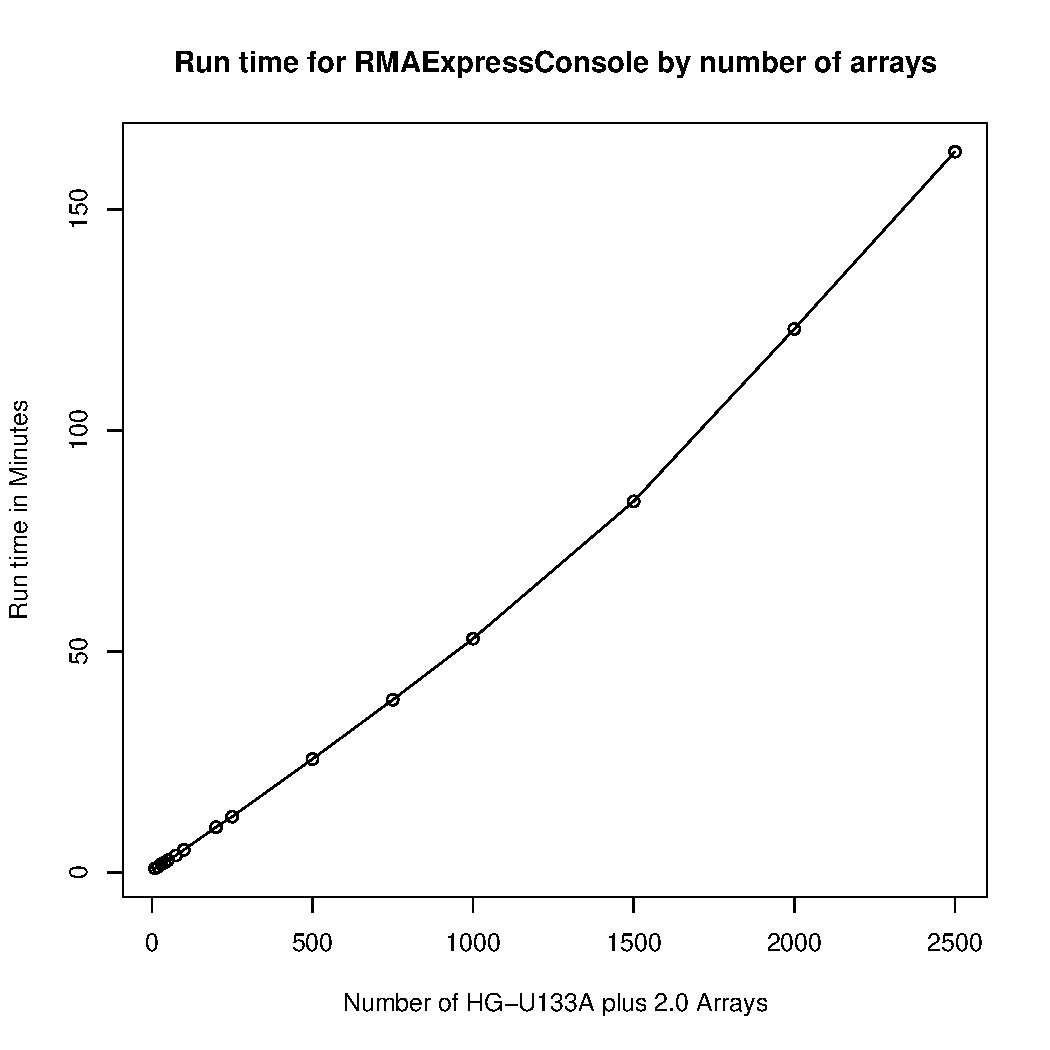
\includegraphics[width=4in,height=4in]{Runtimes.pdf}
\caption{Running times using RMAExpressConsole 1.0 Release} \label{timingtest}
\end{figure}

The amount of time it will take to process a set of CEL files and process them to RMA expression values depends on a number of factors including:
\begin{itemize}
\item Number of probes and probesets on the chip
\item Number of CEL files
\item Configuration of computer including processor speed, amount of RAM, operating system.
\item Configuration of RMAExpress (or RMAExpressConsole)
\end{itemize}

A set of timing tests were run using RMAExpressConsole 1.0 on a machine with the following basic configuration:
\begin{itemize}
\item Version: RMAExpressConsole 1.0 with version 2 output file but no output of plots
\item OS: Fedora Core 9 x86\_64 Linux running kernel 2.6.25.6-55.fc9.x86\_64
\item Processor: AMD Athlon X2 5600+ 
\item RAM: 8 GB DDR2 PC6400
\item Chip type: HGU-133A Plus 2.0
\item Number of CEL files: Varied from 10 to 2500
\item Buffer size: 1 arrays, 25000 probes 
\item Timing: done using the shell command time and the output ``Real''.
\end{itemize}
with the results shown in Figure \ref{timingtest}. It can be seen from this plot that, at least for this range of the number of CEL files, the processing time is roughly linear. The largest dataset run was 2500 CEL files and had a total running of approximately 163 minutes. This highlights the relative efficiency of RMAExpress and its ability to handle extremely large datasets.


  
\end{document}
